\chapter{Differential equations of mass, momentum and energy}
In order to understand a fluid flow completely, we want to know:
\begin{itemize}[noitemsep]
  \item Velocity Field
  \item Pressure
  \item Density
  \item Temperature
\end{itemize}
at any time ($t$) and any place ($x,y,z$). All the variables mentioned are going to be a function of space and time. A mathematical model, based on the mass-conservation equation and momentum-conservation equation, will be formulated to obtain the flow around an object.
\subsubsection{List of Variables:}
\begin{center}
  \begin{tabular}{ |c|c|c|c|c| }
    \hline
    Name          & Variable                                      & Type   & Unit                             & Variables \\
    \hline
    Velocity      & $\vec{V} = u\hat{i}+v\hat{j}+w\hat{k}$        & Vector & (\si{\meter\per\second})         & 3         \\
    \hline
    Pressure      & $p$                                           & Scalar & (\si{\newton\per\meter\squared}) & 1         \\
    \hline
    Temperature   & $T$                                           & Scalar & (\si{\celsius})                  & 1         \\
    \hline
    Density       & $\rho$                                        & Scalar & (\si{\kilogram\per\meter\cubed}) & 1         \\
    \hline
    Stress Tensor & $T = \left[ \begin{array}{ccc} \tau_{xx} & \tau_{xy} & \tau_{xz} \\ \tau_{yx} & \tau_{yy} & \tau_{yz} \\ \tau_{zx} & \tau_{zy} & \tau_{zz} \end{array}\right]$ &        & (\si{\newton\per\meter\squared}) & 6         \\
    \hline
  \end{tabular}
\end{center}
For most of this course, the fluid will be assumed to be incompressible. Hence, the $\rho$ will stay constant most of the time. The stress tensor takes into account of the forces which are extered on the surface of an infinitesimal particle. It has 6 variables; those who are on the opposite side of the diagonal (such as $\tau_{xy}$ and $\tau_{yx}$) are the same. Overall, there are 12 variables; hence, 12 equations are needed to fully understand a specific flow.
\section{Conservation of Mass - Continuity Equation}
Control Volume Analysis can be done with the following equation:
\begin{gather}
  \frac{\partial}{\partial t} \int_{V}{\rho dV} + \oint_{S}{\rho \vec{V} \cdot \hat{n}dS} = 0
  \label{conservationofmass}
\end{gather}
The $\frac{\partial}{\partial t} \int_{V}{\rho dV}$ part of the equation describes the mass in the control volume and how it changes with time. \\\\
The $\oint_{S}{\rho \vec{V} \cdot \hat{n}dS}$ part of the equation takes in the account the mass going in and out of the control volume (crossing the control surface). \\\\
The equation is equal to 0 as the mass has to be conserved.
\begin{figure}[H]
  \centering
  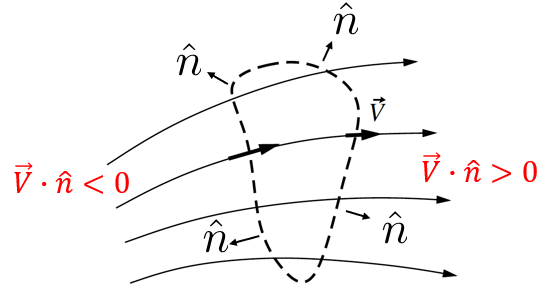
\includegraphics[width = 0.7 \textwidth]{./img/Control Volume.PNG}
  \caption{A control volume with a flow, velocity field $\vec{V}$ and the normal vectors $\hat{n}$}
\end{figure}
On the right side of the control volume, the angle between $\vec{V}$ and $\hat{n}$ is greater than 90$\si{\degree}$. Therefore, $\vec{V} \cdot \hat{n} > 0$, meaning a net mass is going out of the control volume.
On the left side of the control volume, the angle between $\vec{V}$ and $\hat{n}$ is less than 90$\si{\degree}$. Therefore, $\vec{V} \cdot \hat{n} < 0$, meaning a net mass is going into the control volume.
\section{Differential Form of Continuity Equation}
Let us consider an infinitesimally small cube:
\begin{figure}[H]
  \centering
  \includegraphics[width = 0.7\textwidth]{./img/infinitesimalcube.png}
\end{figure}
Consider Term 1 - the mass variation inside the control volume
\begin{gather}
  \frac{\partial \rho}{\partial t} \cdot dV = \frac{\partial \rho}{\partial t} \cdot\dif x \cdot \dif y \cdot \dif z
  \label{massvariation}
\end{gather}
Consider Term 2 - the contribution of mass from the sides of the cube
\subsubsection{$x$ Orthogonal Contribution:}
\begin{figure}[H]
  \centering
  \includegraphics[width = 0.8\textwidth]{./img/infinitesimalcubewithorthox.png}
\end{figure}
Left Side:
\begin{gather}
  \rho \vec{V} \cdot \hat{n} \dif S = \rho \vec{V} \cdot (-\hat{i}) \dif z \dif y\\
  = - \rho u \dif z \dif y
\end{gather}
Right Side:
\begin{gather}
  \left(\rho u + \frac{\partial \rho u}{\partial x} \cdot \dif x \right) \dif z \dif y
\end{gather}
There won't be a negative ($-$) sign as the normal vector and velocity field are moving in the same direction. The $\frac{\partial \rho u}{\partial x} \cdot \dif x$ part comes from the incremental change in mass while moving in the $x$ direction.
The net contribution from the orthogonal $x$ direction is
\begin{gather}
  = \frac{\partial \rho u}{\partial x} \dif x \dif z \dif y
  \label{xorthogonalcontribution}
\end{gather}
\subsubsection{$y$ Orthogonal Contribution:}
\begin{figure}[H]
  \centering
  \includegraphics[width = 0.8\textwidth]{./img/infinitesimalcubewithorthoy.png}
\end{figure}
Front Side:
\begin{align}
  \rho \vec{V} \cdot \hat{n} \dif S & = \rho \vec{V} \cdot (- \hat{j}) \dif x \dif z \\
                                    & = -\rho v \dif x \dif z
\end{align}
Back Side:
\begin{gather}
  \left(\rho v + \frac{\partial \rho v}{\partial y} \cdot \dif y \right) \dif z \dif x
\end{gather}
Final Contribution:
\begin{gather}
  \frac{\partial \rho v}{\partial y} \dif y \dif z \dif x
  \label{yorthogonalcontribution}
\end{gather}
\subsubsection{$z$ Orthogonal Contribution:}
\begin{figure}[H]
  \centering
  \includegraphics[width = 0.35 \textwidth]{./img/infinitesimalcubewithorthoz.png}
\end{figure}
Bottom Side:
\begin{align}
  \rho \vec{V} \cdot \hat{n} \dif S & = \rho \vec{V} \cdot (- \hat{k}) \dif x \dif y \\
                                    & = -\rho w \dif x \dif y
\end{align}
Top Side:
\begin{gather}
  \left(\rho w + \frac{\partial \rho w}{\partial z} \cdot \dif z \right) \dif x \dif y
\end{gather}
Final Contribution:
\begin{gather}
  \frac{\partial \rho w}{\partial z} \dif z \dif x \dif y
  \label{zorthogonalcontribution}
\end{gather}
\subsubsection{Conservation of Mass For an Infinitesimal Volume:}
All of the contributions above (\ref{massvariation}, \ref{xorthogonalcontribution}, \ref{yorthogonalcontribution}, \ref{zorthogonalcontribution}) are added up and the conservation of mass equation (\ref{conservationofmass}) becomes:
\begin{gather}
  \frac{\partial \rho}{\partial t} \cdot\dif x \cdot \dif y \cdot \dif z + \frac{\partial \rho u}{\partial x} \dif x \dif z \dif y + \frac{\partial \rho v}{\partial y} \dif y \dif z \dif x + \frac{\partial \rho w}{\partial z} \dif z \dif x \dif y = 0
\end{gather}
This simplifies to:
\begin{equation}
  \frac{\partial \rho}{\partial t} + \frac{\partial \rho u}{\partial x} + \frac{\partial \rho v}{\partial y} + \frac{\partial \rho w}{\partial z} = 0
\end{equation}
We can simplify this a bit more by introducing a term called the \textbf{divergence}.
\begin{equation}
  \frac{\partial \rho}{\partial t} + \nabla \cdot (\rho \vec{V}) = 0
\end{equation}
Where $\nabla \cdot (\rho \vec{V})$ is the divergence of the vector $\rho \vec{V}$. It is a scalar.
\begin{equation}
  \frac{\partial \rho}{\partial t} + \vec{V}\cdot \nabla \rho + \rho \nabla \cdot \vec{V} = 0
\end{equation}
$\nabla \cdot \vec{V}$ is the divergence of the vector $\vec{V}$ and it is a scalar. $\nabla \rho$ is the gradient of the density $\rho$ and is a vector. It can be expanded as:
\begin{equation}
  \nabla \rho = \frac{\partial \rho}{\partial x} \hat{i} + \frac{\partial \rho}{\partial y} \hat{j} + \frac{\partial \rho}{\partial z} \hat{k}
\end{equation}
\begin{gather}
  \vec{V} \cdot \rho \nabla = (u \hat{i} + v \hat{j} + w \hat{k}) \cdot \left( \frac{\partial \rho}{\partial x} \hat{i} + \frac{\partial \rho}{\partial y} \hat{j} + \frac{\partial \rho}{\partial z} \hat{k} \right) = u \frac{\partial \rho}{\partial x} + v \frac{\partial \rho}{\partial y} + w \frac{\partial \rho}{\partial z}\\
  \rho \nabla \cdot \vec{V} = \rho \left( \frac{\partial u}{\partial x} + \frac{\partial v}{\partial y} + \frac{\partial w}{\partial z} \right)
\end{gather}
For steady flow:
\begin{equation}
  \frac{\partial \rho}{\partial t} = 0 \rightarrow \nabla \cdot (\rho \vec{V}) = 0
\end{equation}
For incompressible flow, the density is constant. This means all derivatives of $\rho$ are 0. Hence, our equation reduces to:
\begin{equation}
  \rho = \textrm{const} \rightarrow \nabla \cdot \vec{V} = \frac{\partial u}{\partial x} + \frac{\partial v}{\partial y} + \frac{\partial w}{\partial z} = 0
  \label{velocitydivergence}
\end{equation}
Each of these derivatives represent the stretch or compression of the fluid particle in the orthogonal direction. When these are all added up, it gives the variation in volume. If this is positive, it shows that the volume has increased with time. If $\rho$ is constant, then the volume cannot change. Which is why equation (\ref{velocitydivergence}) must equal 0.
\section{Conservation of Momentum}
\begin{equation}
  \frac{\partial}{\partial t} \int_V \rho \vec{V} \dif V + \oint_S \rho \vec{V}(\vec{V} \cdot \hat{n}) \dif S = \sum \vec{F}
  \label{conservationofmomentum}
\end{equation}
We have two types of external force that can act on our infinitesimal fluid element, \textbf{volumetric} forces (e.g. gravity) and \textbf{surface} forces (shear, pressure). The 2 terms of the conservation of momentum equation are investigated. In the example below, only the momentum in the $x$ direction is being looked into. \\\\
Consider Term 1 - the momentum in 3D changing with time
\begin{figure}[H]
  \centering
  \includegraphics[width = 0.7 \textwidth]{./img/momentuminx.png}
\end{figure}
\begin{gather}
  \frac{\partial}{\partial t} \int_V \rho \vec{V} \dif V = \frac{\partial \rho u}{\partial t}\dif x \dif y \dif z
  \label{momentumin3d}
\end{gather}
Consider Term 2 - the flux of momentum through the sides of the control volume \\
\subsubsection{Momentum Contribution in $x$ Entering from $x$ Orthogonal:}
\begin{figure}[H]
  \centering
  \includegraphics[width = 0.8 \textwidth]{./img/fluxinx.png}
\end{figure}
Left Side:
\begin{gather}
  -(\rho u^2)\dif y \dif z
\end{gather}
Right Side:
\begin{gather}
  \left(\rho u^2 + \frac{\partial \rho u^2}{\partial x} \dif x \right) \dif y \dif z
\end{gather}
Final Contribution:
\begin{equation}
  \frac{\partial (p u^2)}{\partial x} \dif x \dif y \dif z
  \label{xmomentumcontribution}
\end{equation}
\subsubsection{Momentum Contribution in $x$ Entering from $z$ Orthogonal:}
\begin{figure}[H]
  \centering
  \includegraphics[width = 0.45 \textwidth]{./img/fluxthroughxy.png}
\end{figure}
Bottom Side:
\begin{gather}
  -(\rho u w) \dif x \dif y
\end{gather}
Top Side:
\begin{gather}
  \left(\rho u w + \frac{\partial \rho u w}{\partial z} \dif z \right) \dif x \dif y
\end{gather}
Final Contribution:
\begin{equation}
  \frac{\partial (\rho u w)}{\partial z} \dif x \dif y \dif z
  \label{zmomentumcontribution}
\end{equation}
\subsubsection{Momentum Contribution in $x$ Entering from $y$ Orthogonal:}
\begin{figure}[H]
  \centering
  \includegraphics[width = 0.8 \textwidth]{./img/fluxthroughxz.png}
\end{figure}
Front Side:
\begin{gather}
  -(\rho u v) \dif x \dif z
\end{gather}
Back Side:
\begin{gather}
  \left(\rho u v + \frac{\partial \rho u v}{\partial y} \dif y \right) \dif x \dif z
\end{gather}
Final Contribution:
\begin{equation}
  \frac{\partial \rho u v}{\partial y} \dif x \dif y \dif z
  \label{ymomentumcontribution}
\end{equation}
\subsubsection{All Momentum Contributions:}
All of the contributions above (\ref{momentumin3d}, \ref{xmomentumcontribution}, \ref{ymomentumcontribution}, \ref{zmomentumcontribution}) are added up and the conservation of momentum equation (\ref{conservationofmomentum}) becomes:
\begin{equation}
  \frac{\partial \rho u}{\partial t}\dif x \dif y \dif z + \frac{\partial(\rho u^2)}{\partial x} \dif x \dif y \dif z + \frac{\partial (\rho u w)}{\partial z} \dif x \dif y \dif z + \frac{\partial \rho u v}{\partial y} \dif x \dif y \dif z = \sum \vec{F}
\end{equation}
Consider Term 3 - $\sum \vec{F}$ term. \\\\
Pressure is always exerted orthogonal to a face. We also have our $\tau$ stresses acting orthogonally. In the example below, some steps of calculations are skipped (can still be viewed on the figures); only the final contributions on each direction are shown.
\subsubsection{$x$ Orthogonal Shear Force}
\begin{figure}[H]
  \centering
  \includegraphics[width = 0.6 \textwidth]{./img/forcesinx.png}
\end{figure}
\begin{equation}
  - \left( \frac{\partial p}{\partial x} \right) \dif x \dif y \dif z + \left( \frac{\partial \tau_{xx}}{\partial x} \right) \dif x \dif y \dif z
\end{equation}
\subsubsection{$z$ Orthogonal Shear Force}
\begin{figure}[H]
  \centering
  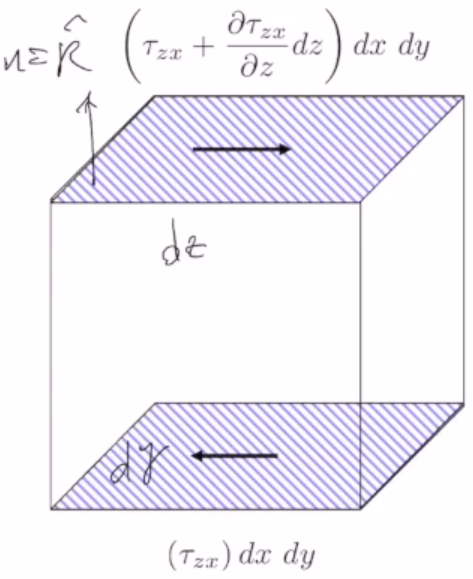
\includegraphics[width = 0.3 \textwidth]{./img/forceinxz.png}
\end{figure}
\begin{equation}
  \left( \frac{\partial \tau_{zx}}{\partial z} \right) \dif x \dif y \dif z
\end{equation}
\subsubsection{$y$ Orthogonal Shear Force}
\begin{figure}[H]
  \centering
  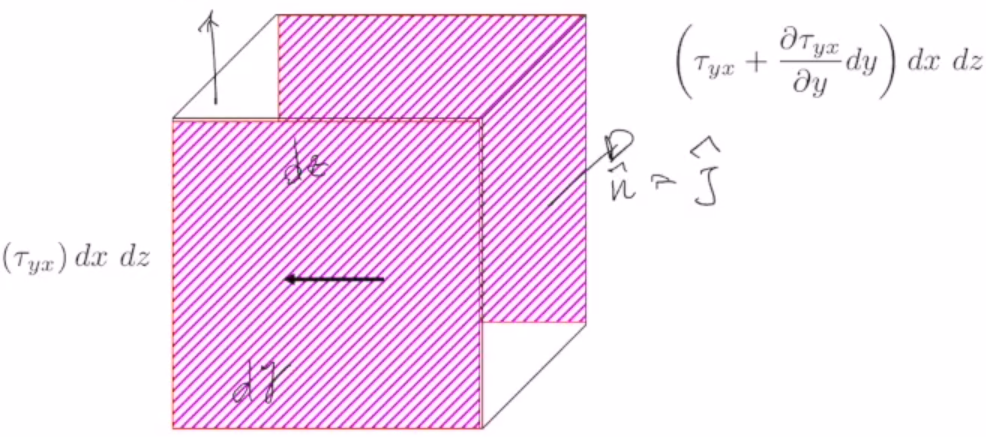
\includegraphics[width = 0.6 \textwidth]{./img/forceinxy.png}
\end{figure}
\begin{equation}
  \left( \frac{\partial \tau_{yx}}{\partial y} \right) \dif x \dif y \dif z
\end{equation}
\subsubsection{Sum of the Forces $\sum \vec{F}$}
\begin{multline}
  \sum F_x = - \left( \frac{\partial p}{\partial x} \right) \dif x \dif y \dif z + \left( \frac{\partial \tau_{xx}}{\partial x} \right) \dif x \dif y \dif z + \\ \left( \frac{\partial \tau_{zx}}{\partial z} \right) \dif x \dif y \dif z + \left( \frac{\partial \tau_{yx}}{\partial y} \right) \dif x \dif y \dif z
\end{multline}
\subsubsection{Conservation of Momentum Equations in All Directions}
Combining Term 1, Term 2 and Term 3 from above yields the following equations for the conservation of momentum in 3D. \\\\
\textbf{$x$ Direction:}
\begin{equation}
  \frac{\partial}{\partial t} (\rho u ) + \frac{\partial}{\partial x} (\rho uu) + \frac{\partial}{\partial y} (\rho uv) + \frac{\partial}{\partial z} (\rho uw) = -\frac{\partial p}{\partial x} + \frac{\partial \tau_{xx}}{\partial x} + \frac{\partial \tau_{yx}}{\partial y} + \frac{\partial \tau_{zx}}{\partial z}
\end{equation}
\textbf{$y$ Direction:}
\begin{equation}
  \frac{\partial}{\partial t} (\rho v ) + \frac{\partial}{\partial x} (\rho vu) + \frac{\partial}{\partial y} (\rho vv) + \frac{\partial}{\partial z} (\rho vw) = -\frac{\partial p}{\partial x} + \frac{\partial \tau_{xy}}{\partial x} + \frac{\partial \tau_{yy}}{\partial y} + \frac{\partial \tau_{zy}}{\partial z}
\end{equation}
\textbf{$z$ Direction:} ($\rho g$ is added here due to the gravitational force acting downwards)
\begin{equation}
  \frac{\partial}{\partial t} (\rho w ) + \frac{\partial}{\partial x} (\rho wu) + \frac{\partial}{\partial y} (\rho wv) + \frac{\partial}{\partial z} (\rho ww) = -\frac{\partial p}{\partial x} - \rho g + \frac{\partial \tau_{xz}}{\partial x} + \frac{\partial \tau_{yz}}{\partial y} + \frac{\partial \tau_{zz}}{\partial z}
\end{equation}
These can be added to find that we arrive with two terms, one being the continuity equation, which must equal 0. To summarise, we have our continuity equation and momentum equations below.
\subsubsection{Conservation of Mass (Continuity Equation)}
\begin{equation}
  \frac{\partial \rho}{\partial t} + \nabla \cdot (\rho \vec{V}) = \frac{\partial \rho}{\partial t} + \frac{\partial \rho u}{\partial x} + \frac{\partial \rho v}{\partial y} + \frac{\partial \rho w}{\partial z} = 0
\end{equation}
\subsubsection{$x$ Direction Momentum}
\begin{equation}
  \rho \left( \frac{\partial u}{\partial t} + u \frac{\partial u}{\partial x} + v \frac{\partial u}{\partial y} + w \frac{\partial u}{\partial z} \right) = -\frac{\partial p}{\partial x} + \frac{\partial \tau_{xx}}{\partial x} + \frac{\partial \tau_{yx}}{\partial y} + \frac{\partial \tau_{zx}}{\partial z}
\end{equation}
\subsubsection{$y$ Direction Momentum}
\begin{equation}
  \rho \left( \frac{\partial v}{\partial t} + u \frac{\partial v}{\partial x} + v \frac{\partial v}{\partial y} + w \frac{\partial v}{\partial z} \right) = -\frac{\partial p}{\partial y} + \frac{\partial \tau_{xy}}{\partial x} + \frac{\partial \tau_{yy}}{\partial y} + \frac{\partial \tau_{zy}}{\partial z}
\end{equation}
\subsubsection{$z$ Direction Momentum}
\begin{equation}
  \rho \left( \frac{\partial w}{\partial t} + u \frac{\partial w}{\partial x} + v \frac{\partial w}{\partial y} + w \frac{\partial w}{\partial z} \right) = -\frac{\partial p}{\partial z} -\rho g + \frac{\partial \tau_{xz}}{\partial x} + \frac{\partial \tau_{yz}}{\partial y} + \frac{\partial \tau_{zz}}{\partial z}
\end{equation}
\section{Stress Tensor Notation}
To identify a stress component we use a double subscript notation (tensor notation). The first subscript indicates the direction of the normal to the plane on which stress acts. Second subscript indicates the direction of the stress. Thus, the symbol $\tau_{ij}$ denotes a stress in $j$ direction on a face normal to the $i$-axis.
\begin{figure}[H]
  \centering
  \includegraphics[width = 0.7 \textwidth]{./img/tensorforces.png}
\end{figure}
The normal stresses two contributions are pressure $p$ and viscous stress $\tau$. Pressure is always negative due to it acting against the surface (if we take the arrow coming out of the surface as positive). $\tau$ accounts for the extra stress coming from viscosity.
\begin{gather}
  \sigma_{xx} = -p + \tau_{xx}\\
  \sigma_{yy} = -p + \tau_{yy}\\
  \sigma_{zz} = -p + \tau_{zz}
\end{gather}
Parts on the opposite sides of a stress tensor are equal.
$$ \tau_{xy} = \tau_{yx}, \ \tau_{xz} = \tau_{zx}, \ \tau_{yz} = \tau_{zy} $$